\section{Results}
\begin{figure}
  \centering
  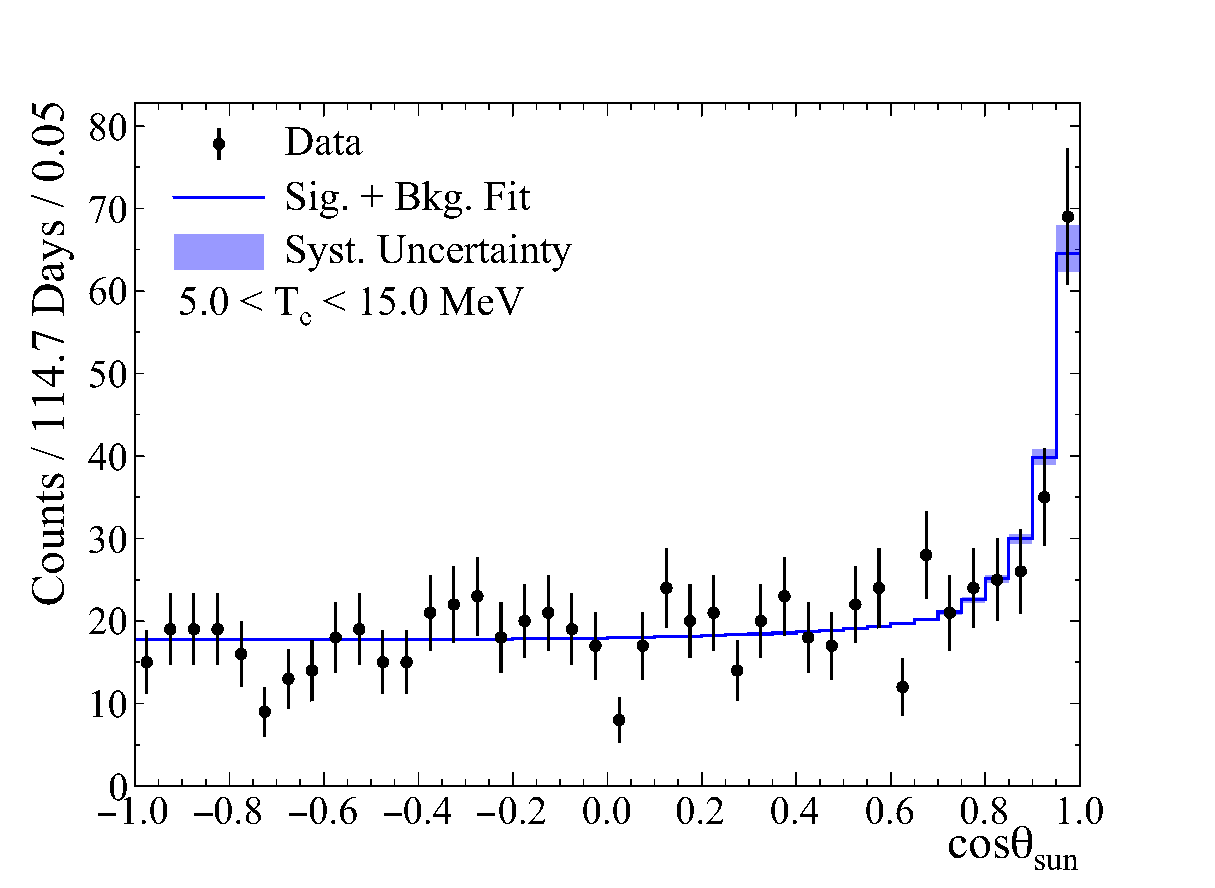
\includegraphics[width=0.7\textwidth]{cos_theta_full}
  \caption[5.0 to 15.0 MeV $\cos\theta_{sun}$ Distribution] {Distribution of event direction
                                              with respect to solar direction.
                                              The systematic error bar includes
                                              angular correlated and
                                              uncorrelated errors.}

  \label{fig:costheta}
\end{figure}
The analysis outline in the previous section was performed in two steps.
First the analysis was done with a single energy bin from $5$ to $15$,
this provided an idea of the signal and background rate, but was not used in
the final flux result.
The principal purpose of the single bin analysis was to constrain the value of
$\delta_{\theta}$, the angular resolution systematic.
A fit was done to this distribution in three dimensions, signal normalization,
background normalization and $\delta_{\theta}$.
In this fit $\delta_{\theta}$ was constrained by the separate $\ce{^{16}N}$ 
results, a bifurcated Gaussian was used to model the likelihood of the
$\ce{^{16}N}$ results.
The fit determined the systematic uncertainty on $\delta_{\theta}$
was determined to be $+0.07$, $-0.12$ a small improvement  compared to the values from the 
$\ce{^{16}N}$ analysis, $+0.08$, $-0.013$.

The analysis was then performed again in six energy bins, five equal width
bins from 5 to 10\,MeV and a single bin from 10 to 15\,MeV.
In each energy bin a two-dimensional fit to the distribution of events in $\cos\theta_{sun}$ was
done to determine the signal and background normalization.
Then the likelihood space from each fit was combined,
marginalizing over each energy bin's background rate,
to find the most likely solar neutrino flux normalization.
The best fit solar rates in each energy bin also serve to provide
a measurement of the spectral shape of the solar neutrino
flux.
The spectral fit was also done as a three-dimensional fit
in each bin, allowing $\delta_{\theta}$ to vary.
This provided negligible difference in the final result
and was significantly more computationally expensive.

For each of these steps the fitting routine was a simple grid scan
over the parameter space. 
The solar and background normalizations were both scanned in $2000$ steps from 0 to
an  value equal to  1.5 times the number of events in the energy bin.
For fits involving $\delta_{\theta}$ 500 steps were used scanning values across
double the $\ce{^{16}N}$ constraint.
The uncertainty introduced by the sampling step size was, in all cases, negligible
compared to the systematic and statistical uncertainty.

Figure~\ref{fig:costheta} shows the distribution of events in $\cos\theta_\text{{sun}}$
for events over the entire energy range of $5$ to $15$\,MeV and the fit to that distribution.\
The value $\delta_\theta$ for the best fit line is fixed to zero, but the 
systematic uncertainties are shown in the blue band.
The fit gives a solar event rate of $1.30\pm0.18$~events/kt-day
 and background rate of  $10.23\pm0.38$~events/kt-day.

From the energy bin-by-bin fit  yielded the best fit solar event rate
as a function of energy shown in Fig~\ref{fig:spectrum}, and
an overall flux
\begin{equation*}
    \Phi_{ES}= 2.53^{+0.31}_{-0.28}\text{(stat.)}^{+0.13}_{-0.10}\text{(syst.)}\times10^6\,\text{cm}^{-2}\text{s}^{-1}\text{.}
\end{equation*}
This value assumes the neutrino flux consists purely of electron flavor neutrinos.\
The result agrees with the elastic scattering flux published by Super-K,
$\Phi_{ES}=\left(2.345\pm0.039\right)\times10^{6}cm^{-2}s^{-1}$~\citep{superk4},
combining statistical and systematic errors.

\begin{figure}
  \centering
  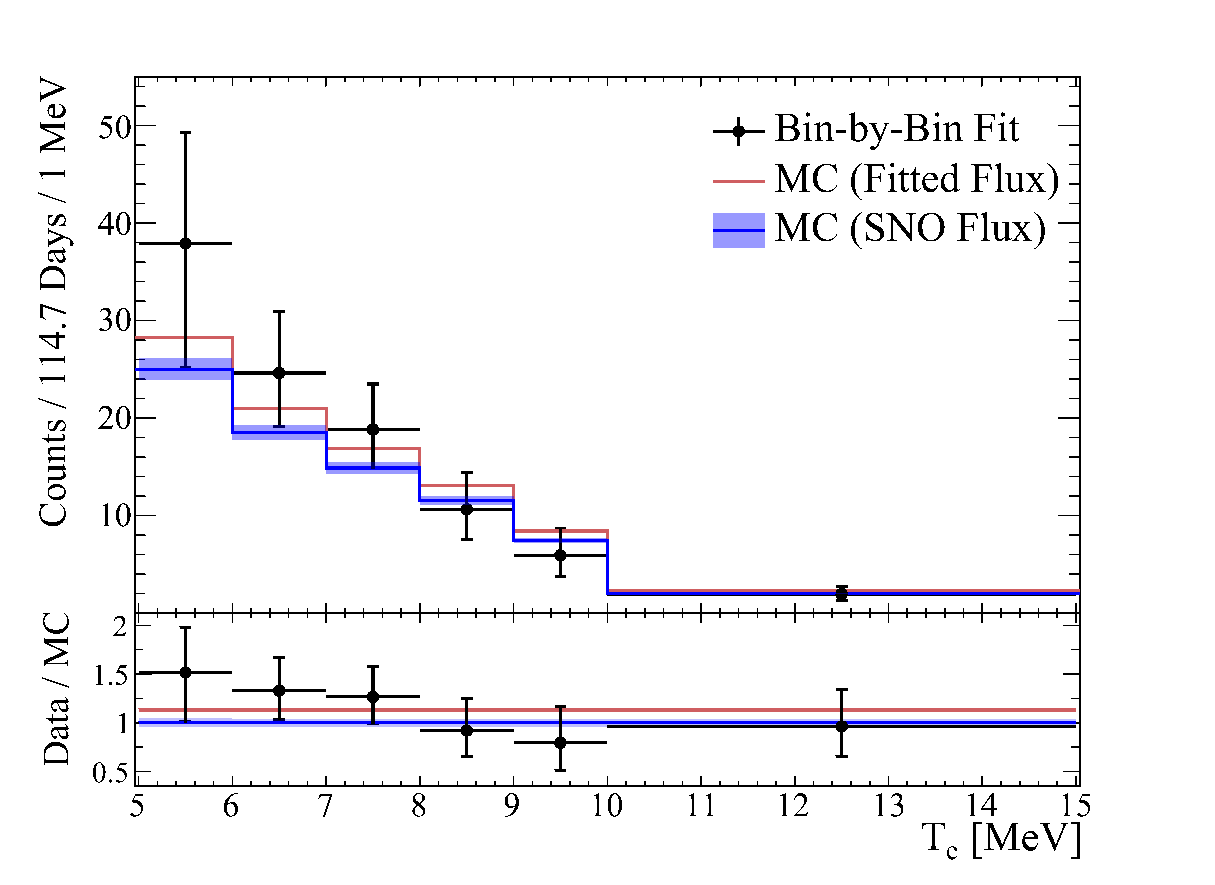
\includegraphics[width=0.7\textwidth]{residual_plot}
  \caption[Solar Spectrum Data to MC Comparison]{
    (Top) The extracted solar neutrino elastic scattering event rate as a
    function of reconstructed electron kinetic energy $T_{\mathrm{e}}$.\
    (Bottom) The same, as a fraction of the expected rate.\
    The red and blue lines show the MC simulation predicted spectrum normalized
    to the best fit flux and the SNO flux measurement~\citep{sno_combined}, respectively.\
    The uncertainty on the SNO result includes reported uncertainty combined with
    mixing parameter uncertainties.\
    The black points are the results of the fits to the $\cos\theta_\text{{sun}}$
    distribution in each energy bin,
    with error bars indicating the combined statistical and systematic
    uncertainty, including energy-correlated uncertainty.\
    A horizontal dash is placed on each error bar indicating the statistics
    only uncertainty; for all points the statistical error is dominant and the systematic
    error bar is not visible above the dash.}
  \label{fig:spectrum}
\end{figure}

\begin{table}
\begin{center}
\begin{tabular}{l c}
\hline
\hline
Systematic & Effect \\
\hline
Energy Scale & 3.9\% \\
Fiducial Volume & 2.8\% \\
Angular Resolution & 1.7\% \\
Mixing Parameters & 1.4\% \\
Energy Resolution & 0.4\% \\
\hline
Total & 5.0\%\\
\hline
\hline
\end{tabular}
\caption{Effect of each systematic uncertainty on the extracted solar neutrino
         flux. Systematic uncertainties with negligible effects
         are not shown. For asymmetric uncertainties, the larger is shown.}
\label{table:systematics}
\end{center}
\end{table}

Including the effects of solar neutrino oscillations, using the neutrino mixing
parameters given in Ref.~\citep{pdg16} and the solar production and electron
density distributions given in Ref.~\citep{bs_ssm} gave a best fit solar flux
of
\begin{equation*}
    \Phi_{\ce{^{8}B}}= 5.95^{+0.75}_{-0.71}\text{(stat.)}^{+0.28}_{-0.30}\text{(syst.)}\times10^{6}\text{cm}^{-2}\text{s}^{-1}\text{.}
\end{equation*}
This result is consistent with the $\ce{^{8}B}$ flux as measured by the SNO experiment,
$\Phi_{\ce{^{8}B}}=\left(5.25\pm0.20\right)\times10^{6}cm^{-2}s^{1}$~\citep{sno_combined}, combining statistical
and systematic uncertainties.\
Figure~\ref{fig:spectrum} shows the best fit solar neutrino $\ce{^{8}B}$ event rate in each
energy bin along with the predicted energy spectrum scaled to the best fit
flux, and scaled to the flux measured by SNO\@. Each statistical error bar on the
measured rate is affected by both the solar neutrino and background rates in that
energy bin.\
Table~\ref{table:systematics} details how each systematic uncertainty affects this result.\

\begin{figure}[htbp]
    \centering
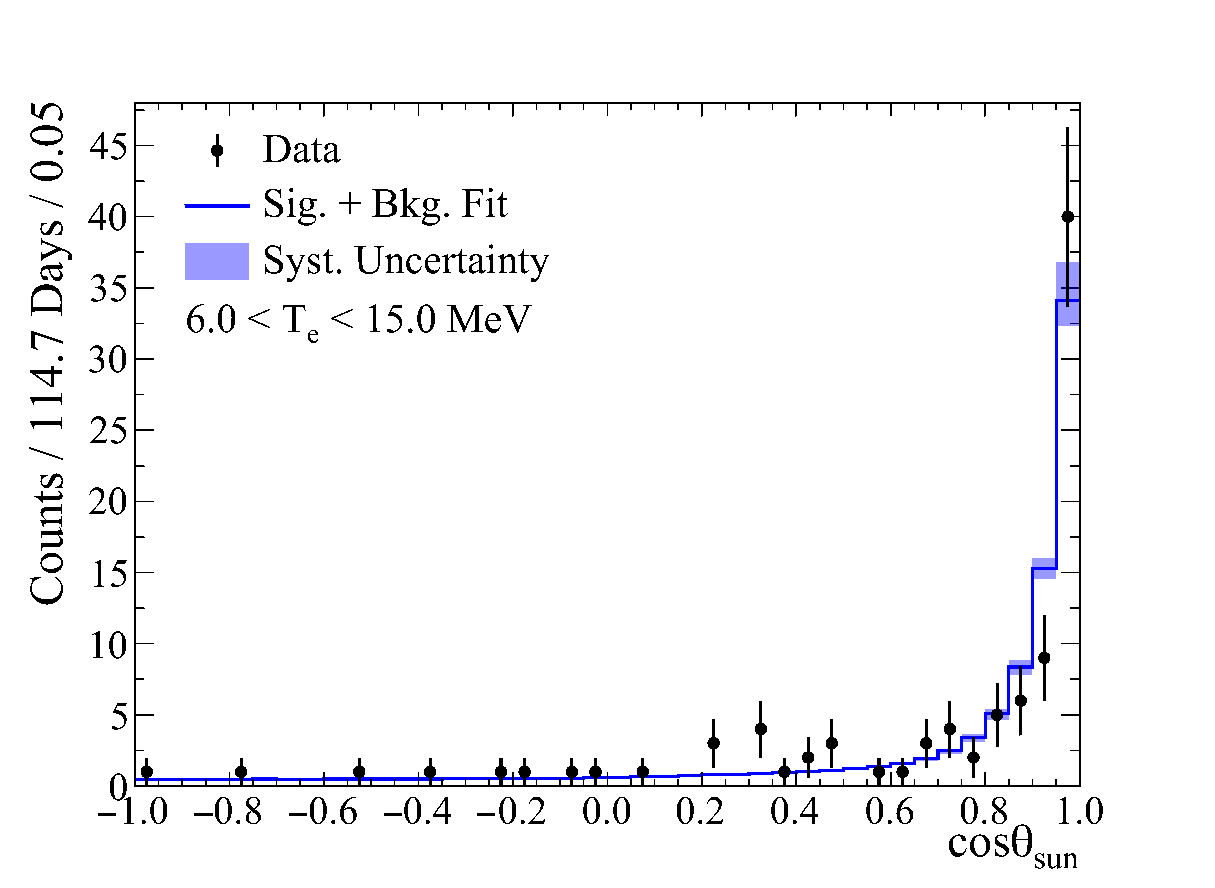
\includegraphics[width=0.7\textwidth]{cos_theta_6mev}%
\caption{Distribution of event directions with respect to solar direction for
    events with energy in \numrange[range-phrase=--]{6.0}{15.0}\,MeV.}
\label{fig:cos_theta_six}
\end{figure}

The upper five energy bins, \numrange[range-phrase=--]{6.0}{15.0}\,MeV, were an
extremely low background region for this analysis.\
There was very little background contamination from
cosmogenically produced isotopes due primarily to depth of the detector.\
The comparatively high rate of backgrounds in the \numrange[range-phrase=--]{5.0}{6.0}\,MeV bin
comes primarily from decays of radioactive isotopes, such as radon, within the detector.\
Figure~\ref{fig:cos_theta_six} shows the distribution in $\cos\theta_\text{{sun}}$ of events at
energies above 6~MeV, illustrating the low background rate.\
In that energy region the best fit background rate was $0.25^{+0.09}_{-0.07}$\,events/kt-day, much
lower than the measured solar rate in that energy range,$1.03^{+0.13}_{-0.12}$\,events/kt-day.
For the region above 6~MeV, this is the lowest
background elastic scattering measurement of solar neutrinos in a water
Cherenkov detector.
Figure~\ref{fig:binbybin} shows the distribution of events in $\cos\theta_{sun}$
with best fit MC prediction in each energy bin of the analysis.

\begin{figure}
\centering
\begin{subfigure}[b]{0.48\textwidth}
\centering
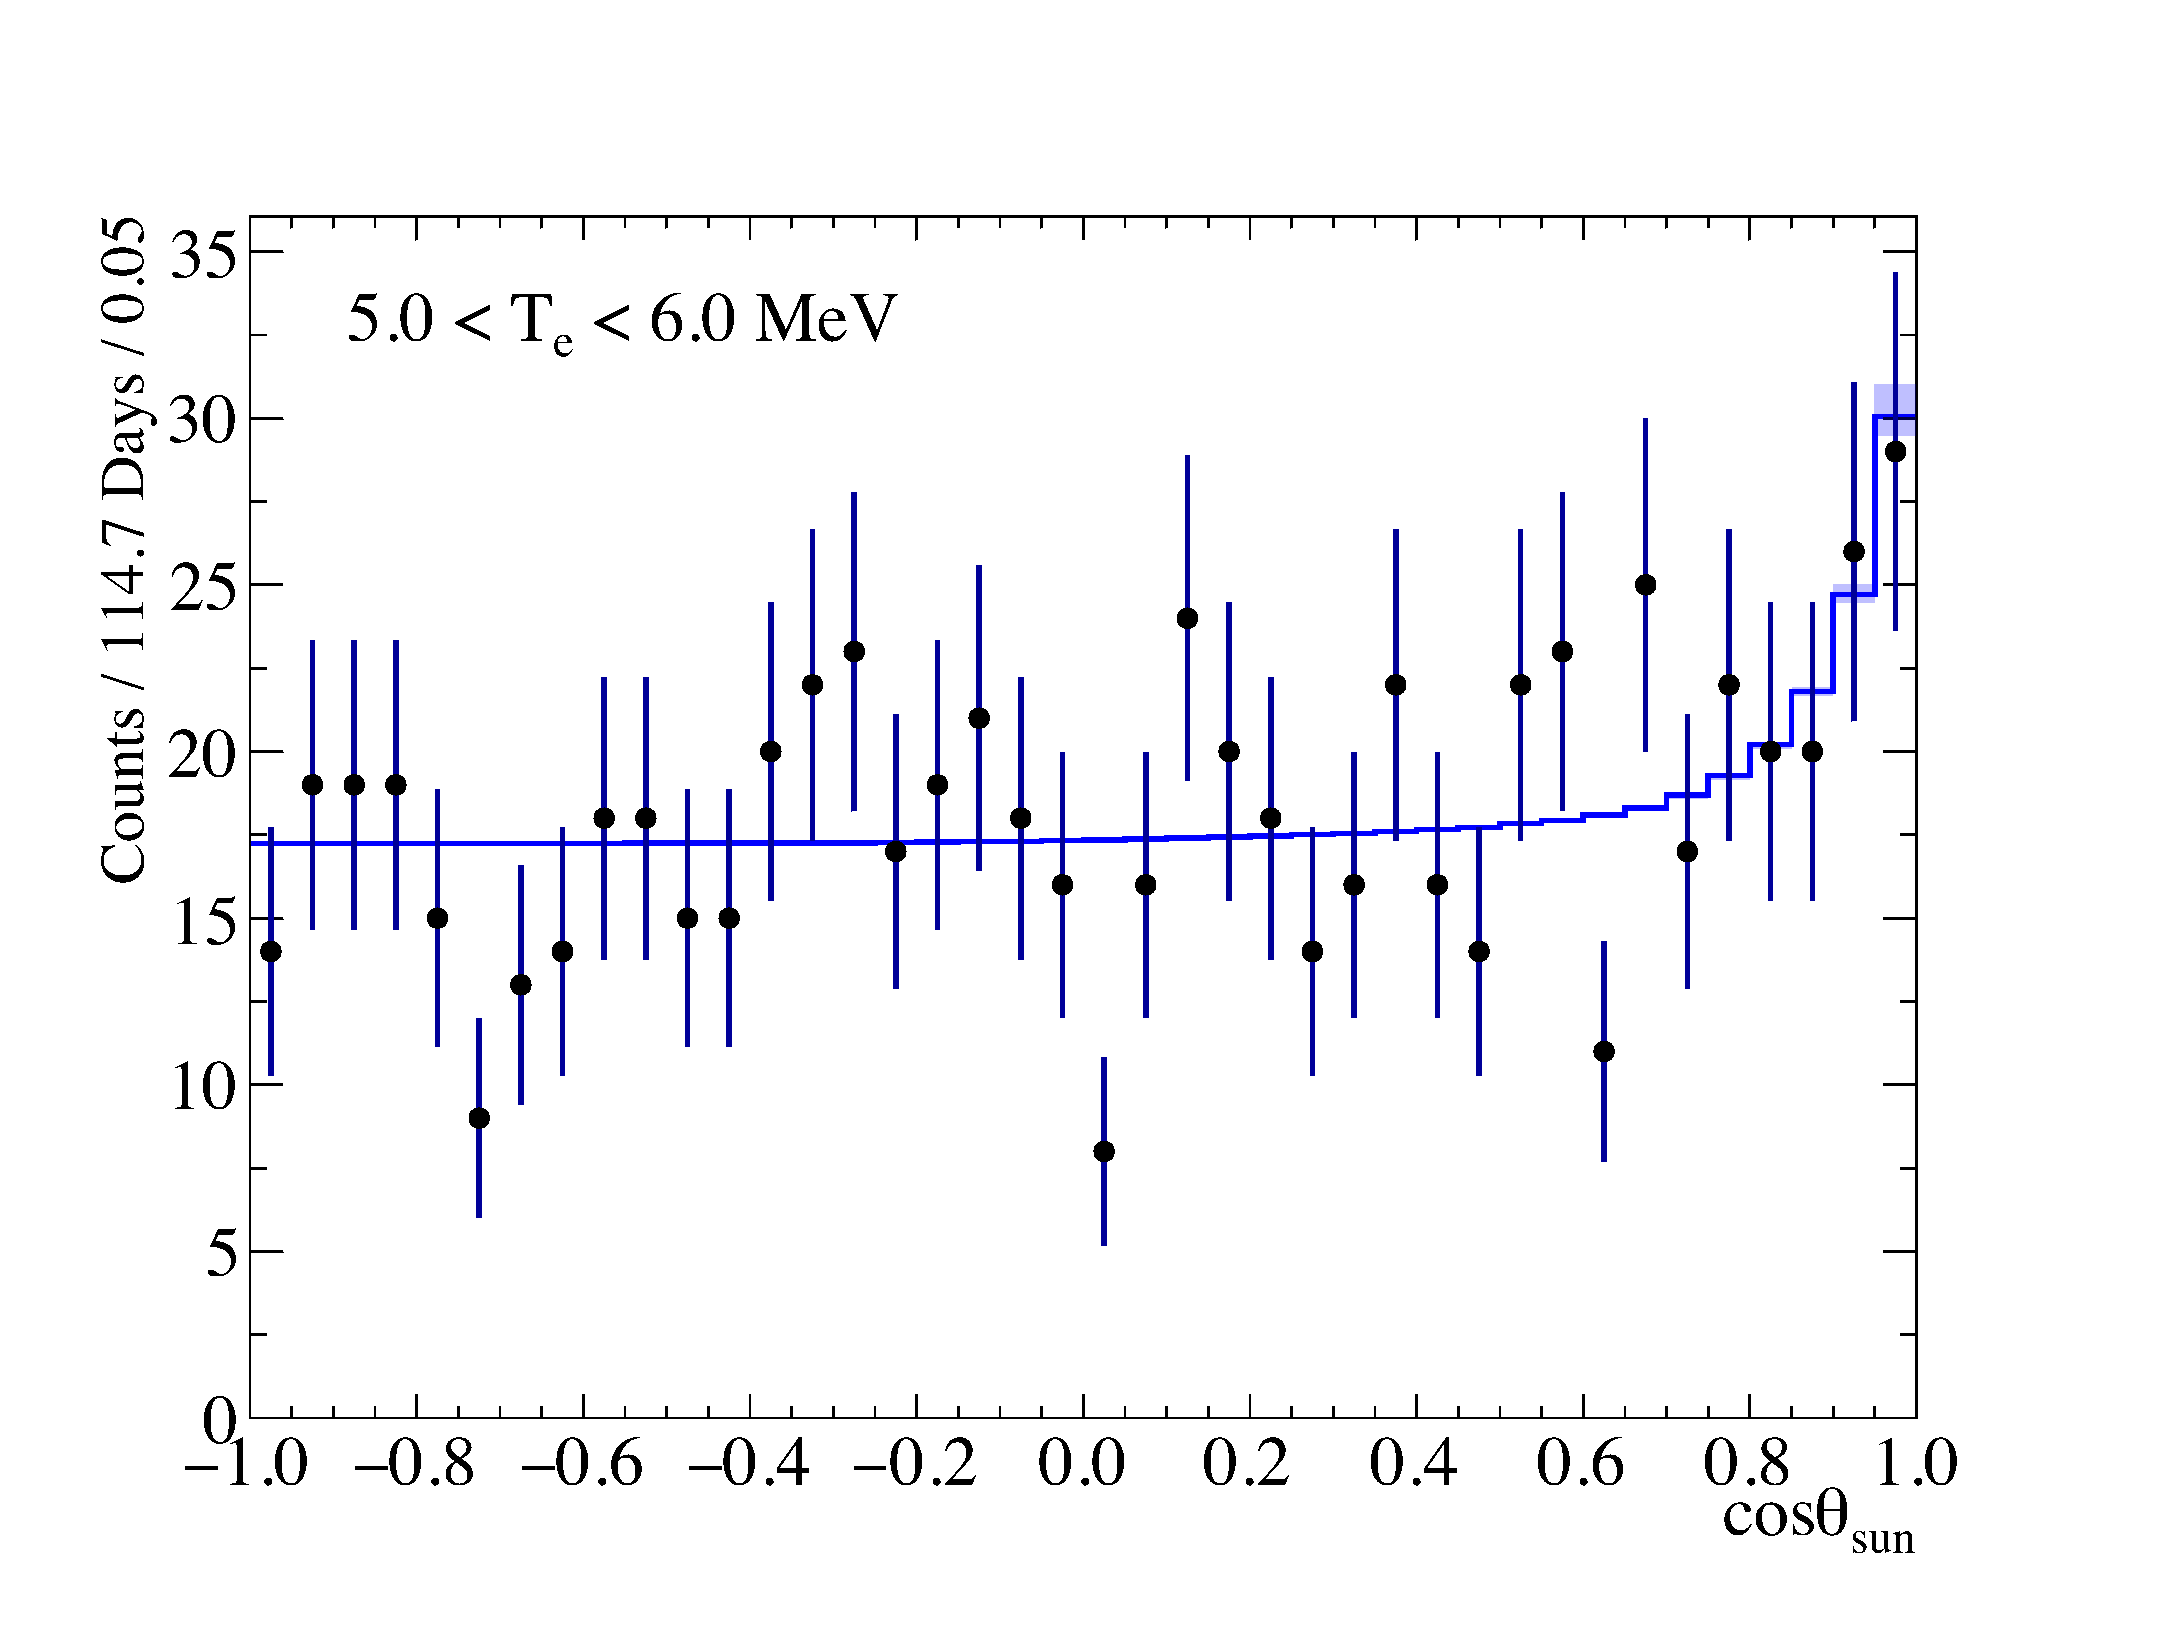
\includegraphics[width=\textwidth]{bin1}
\caption{}
\end{subfigure}
\hfill
\begin{subfigure}[b]{0.48\textwidth}
\centering
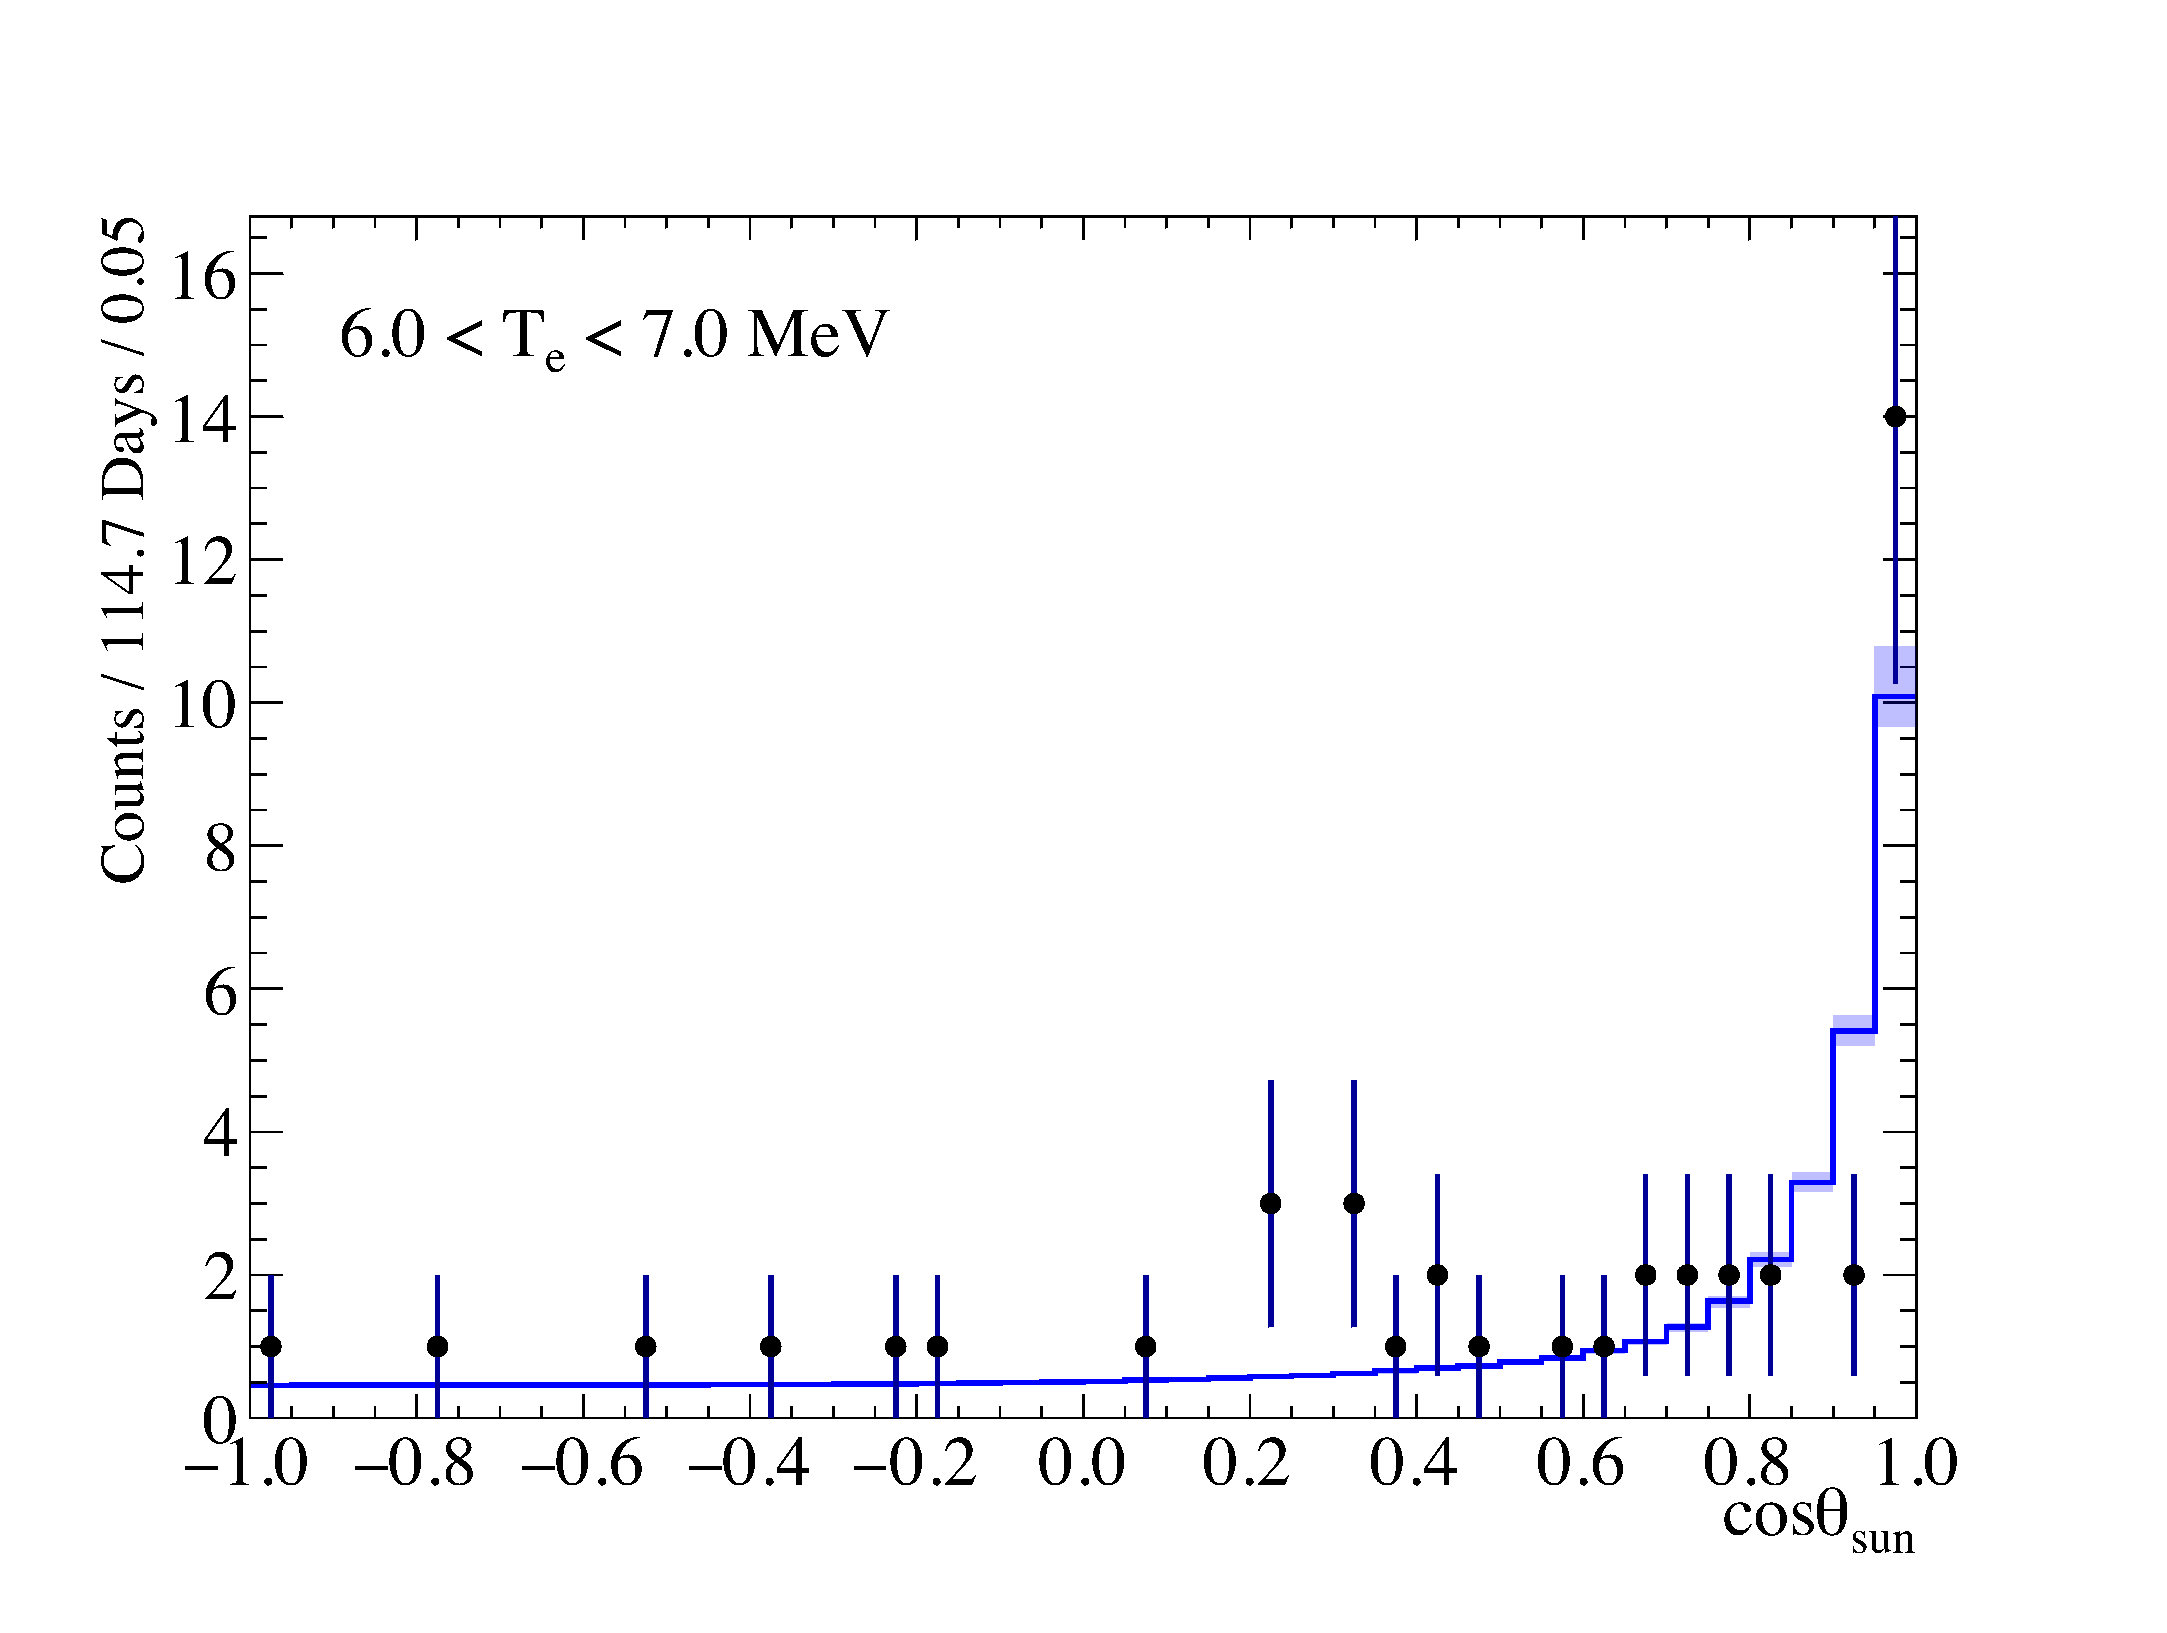
\includegraphics[width=\textwidth]{bin2}
\caption{}
\end{subfigure}

\begin{subfigure}[b]{0.48\textwidth}
\centering
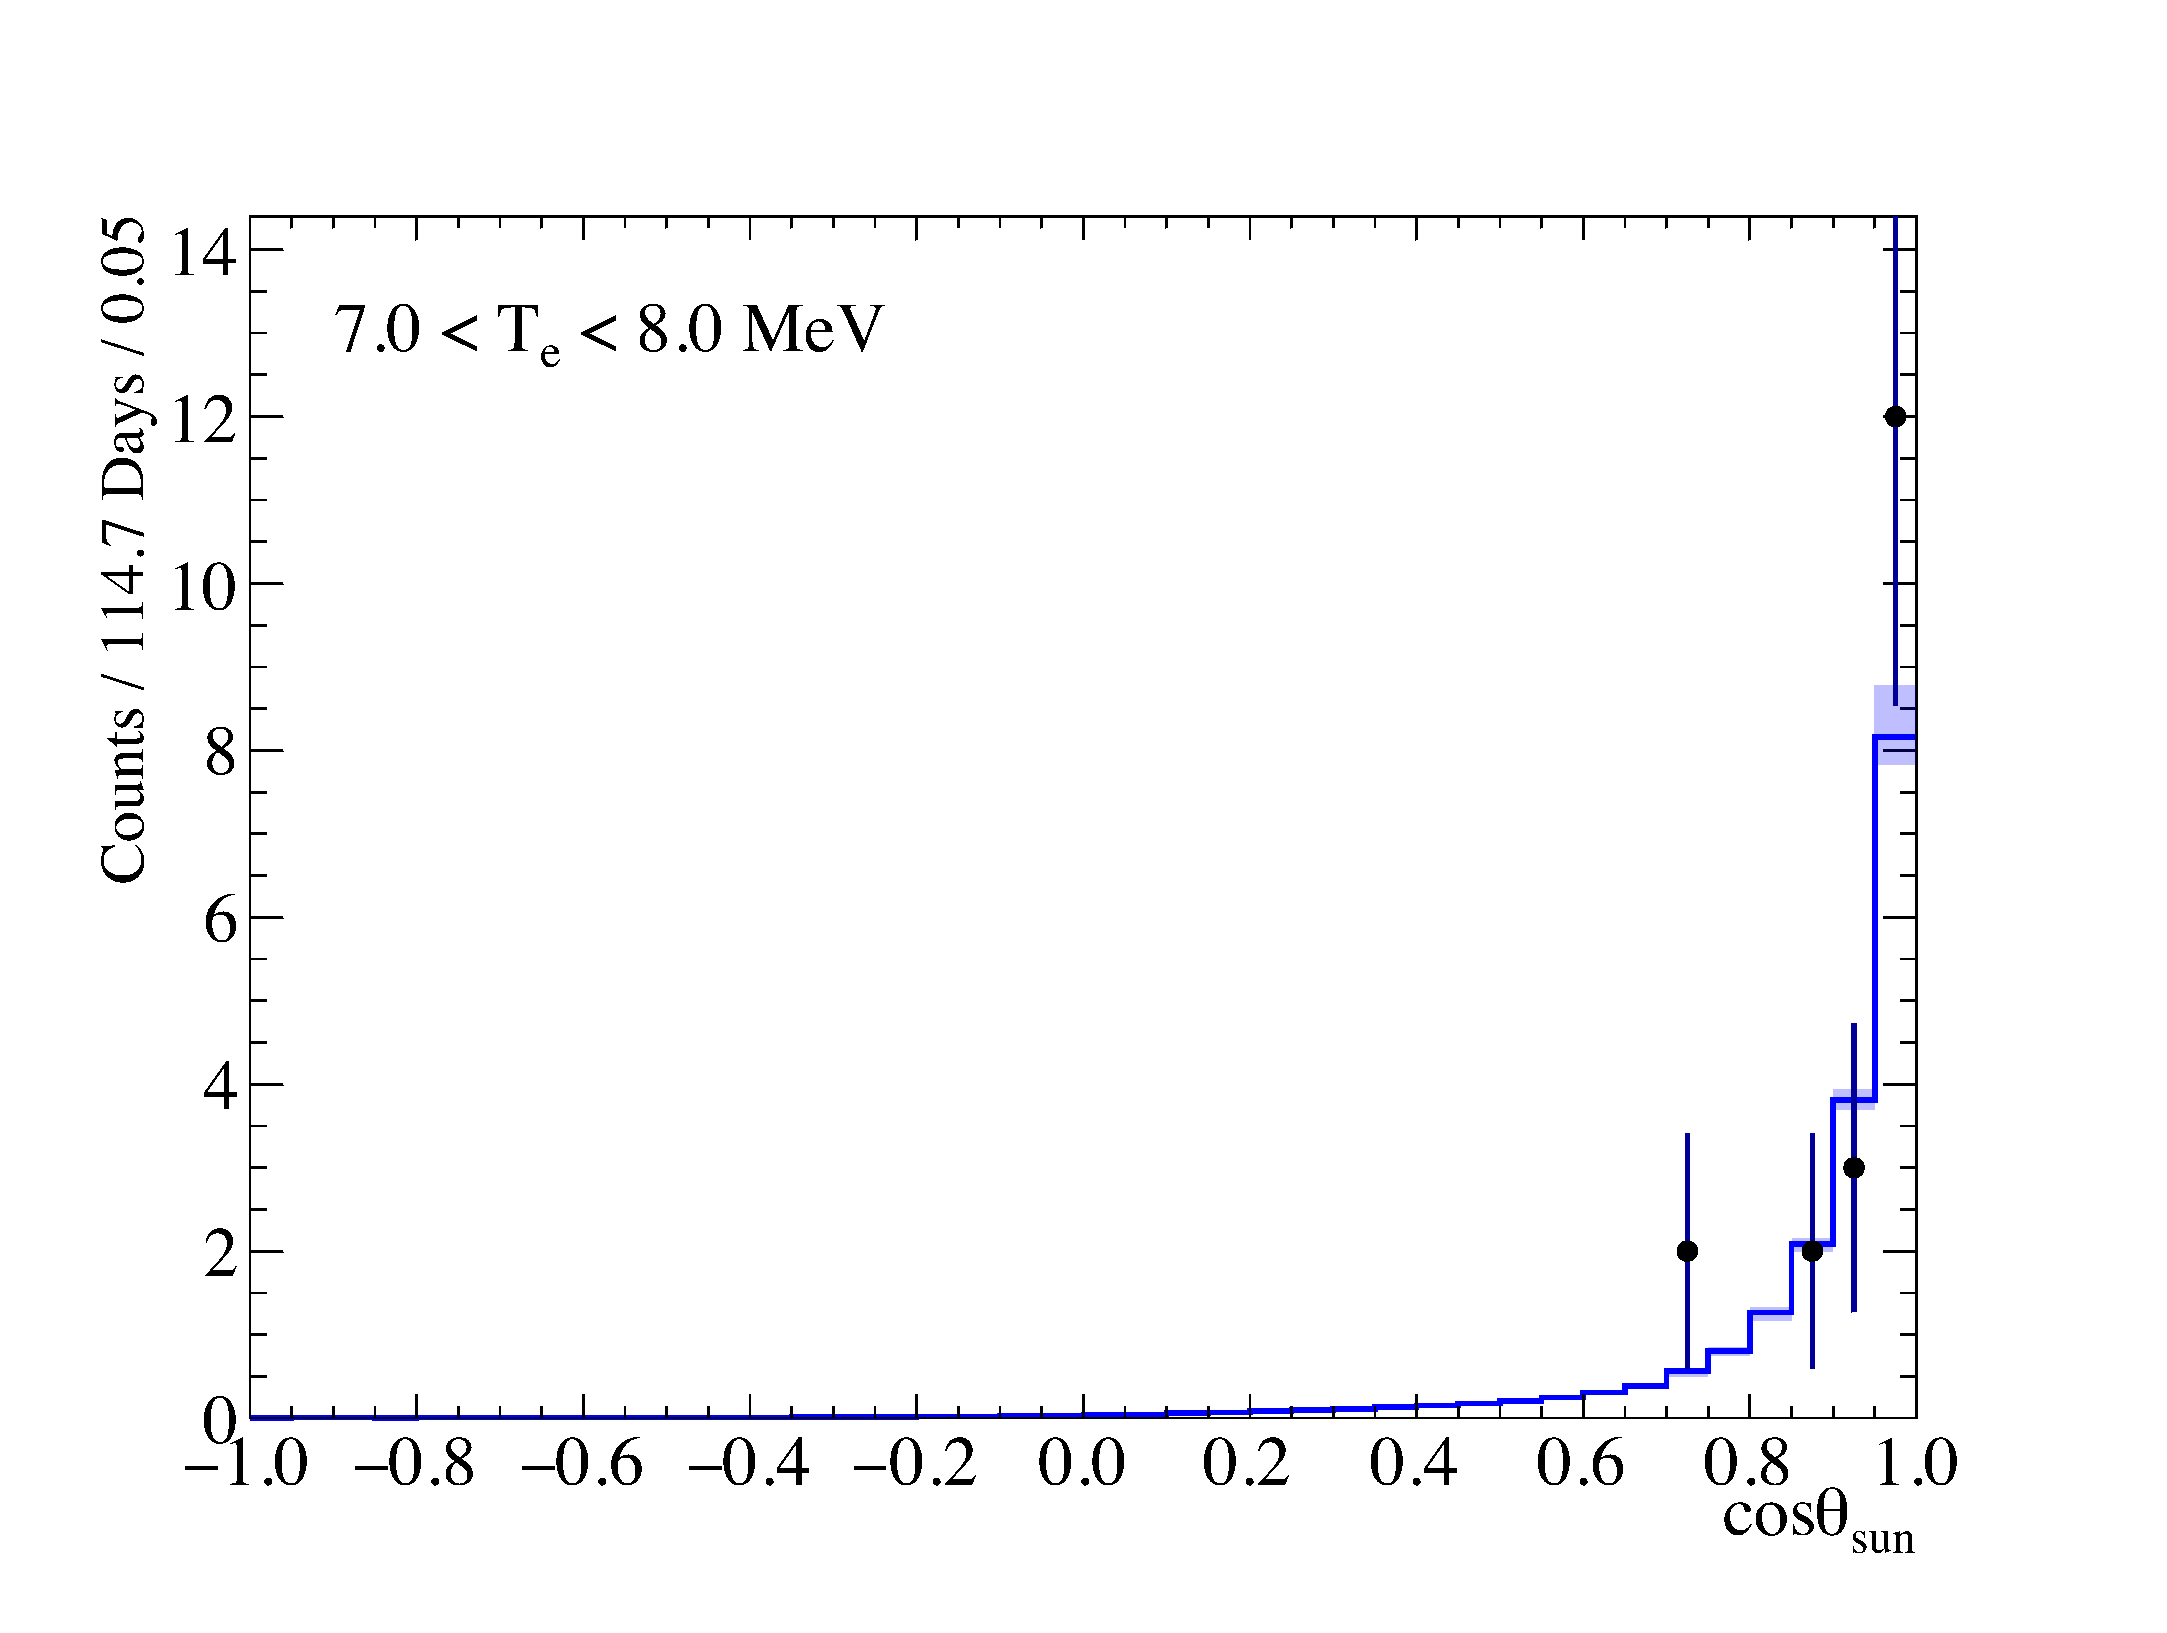
\includegraphics[width=\textwidth]{bin3}
\caption{}
\end{subfigure}
\hfill
\begin{subfigure}[b]{0.48\textwidth}
\centering
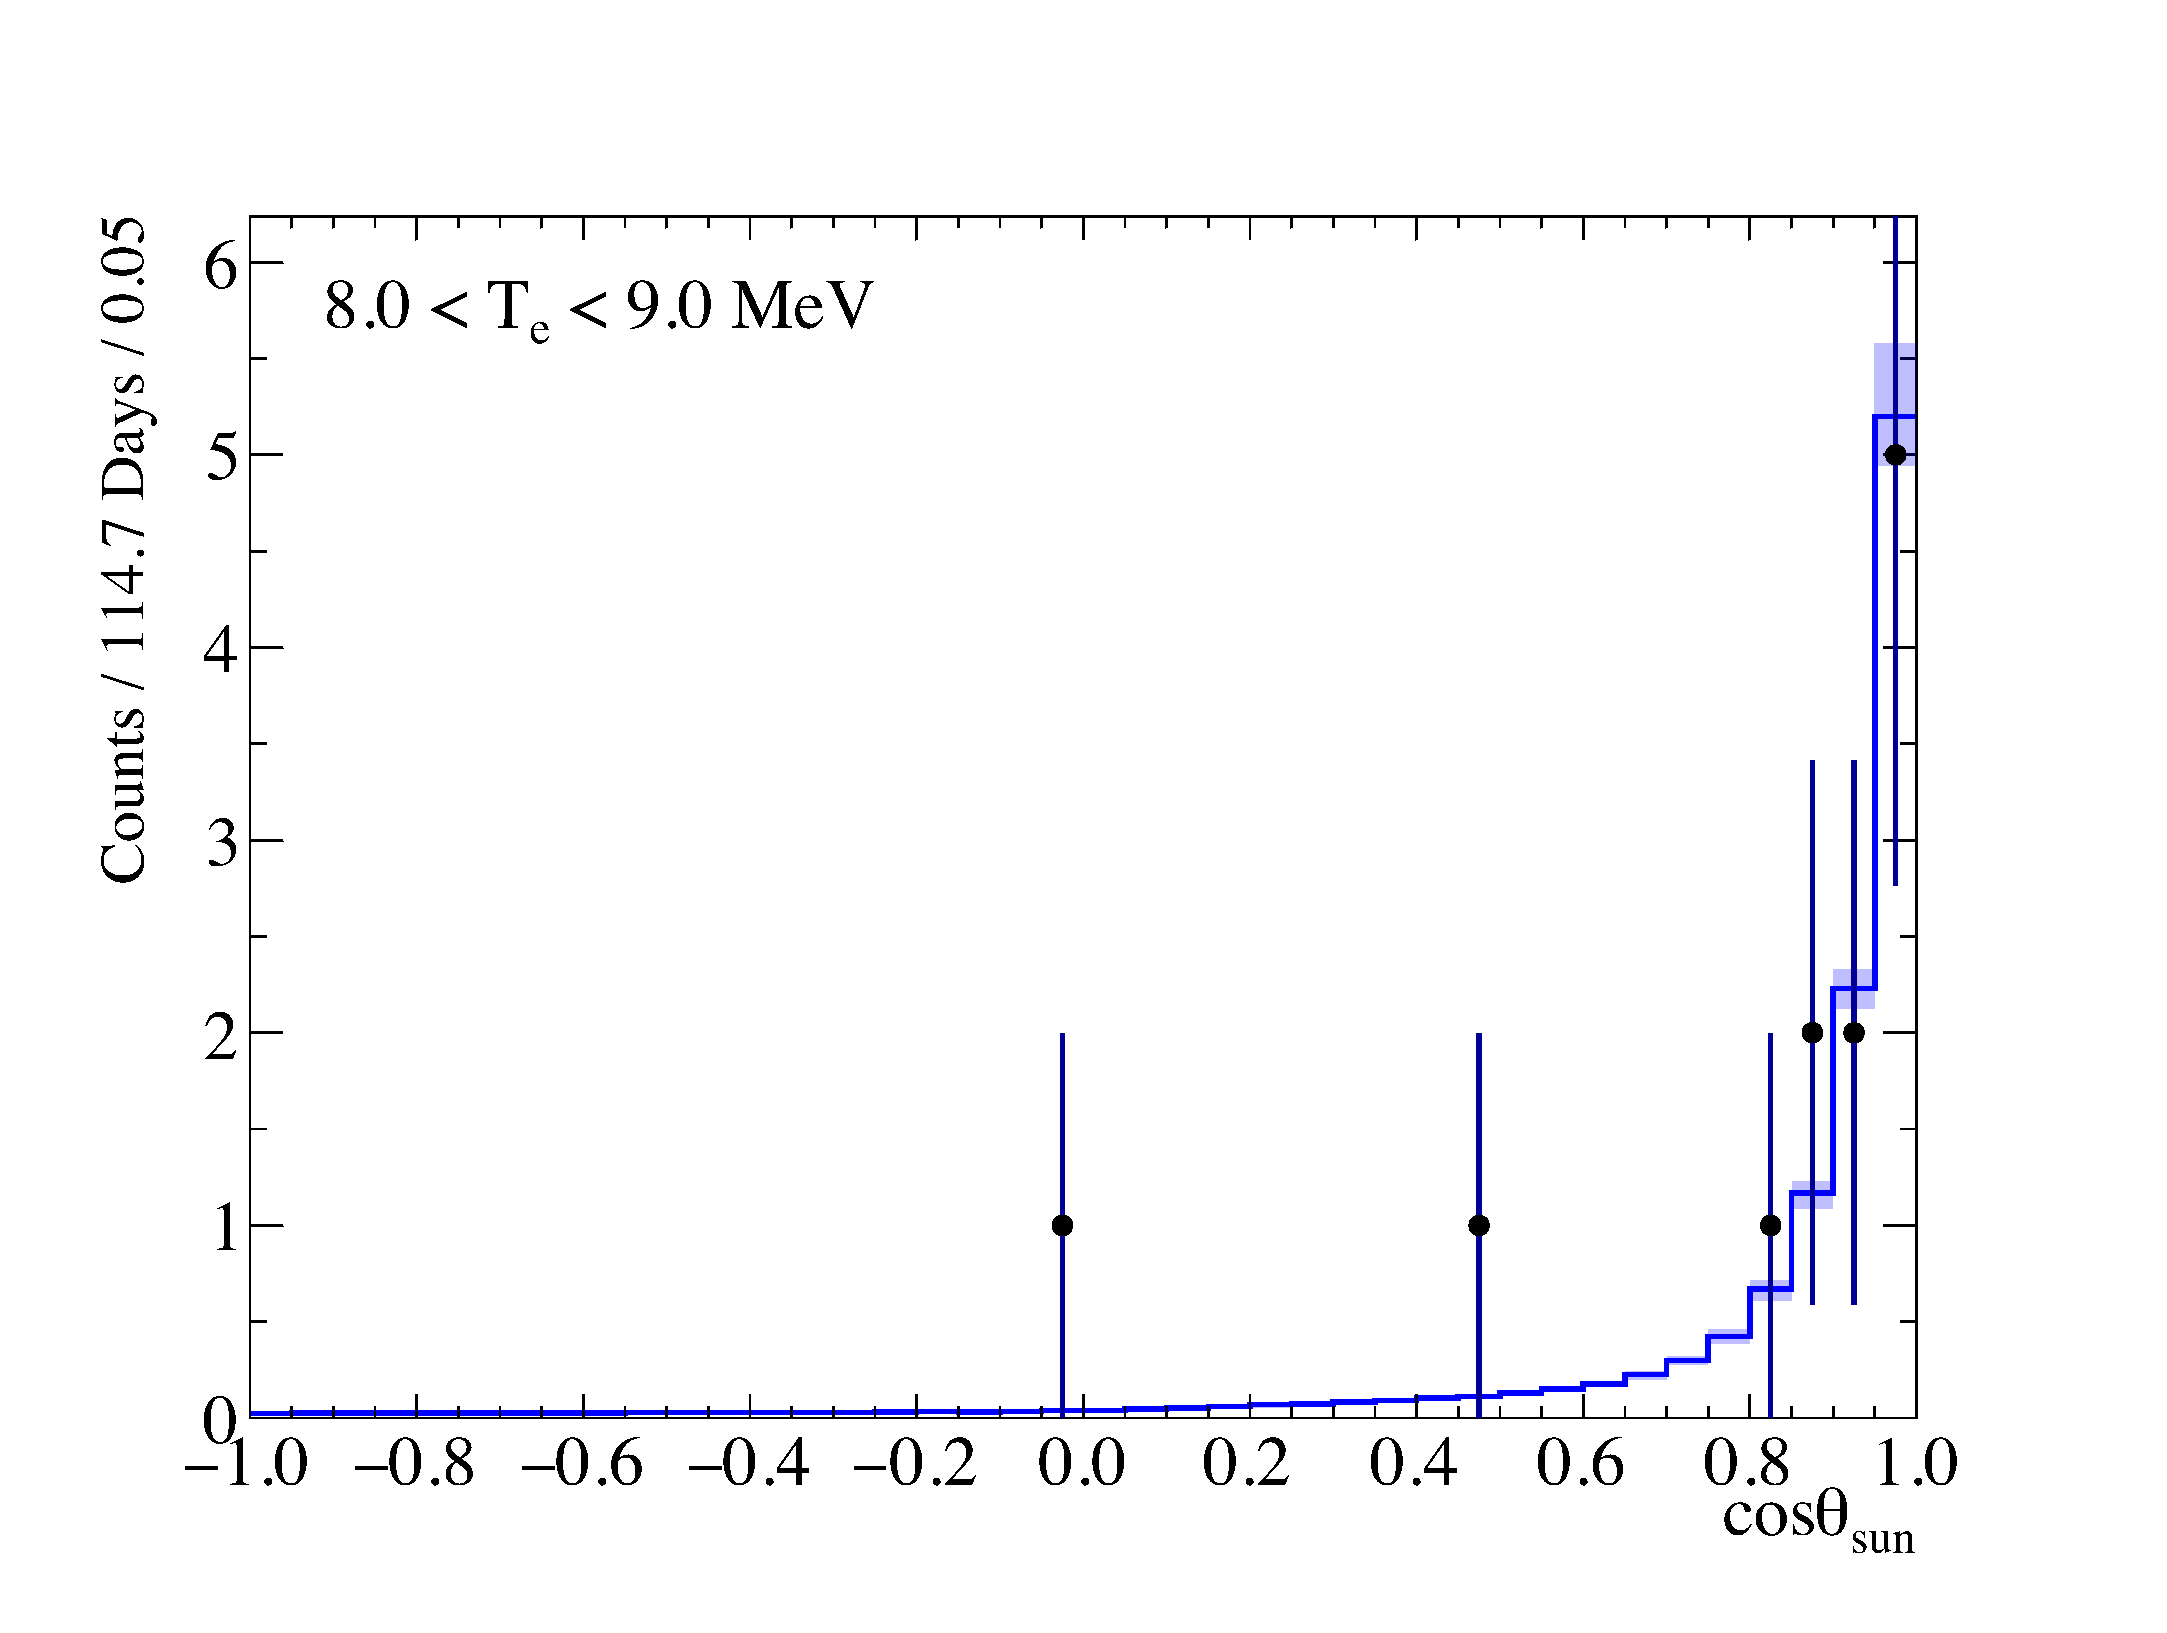
\includegraphics[width=\textwidth]{bin4}
\caption{}
\end{subfigure}

\begin{subfigure}[b]{0.48\textwidth}
\centering
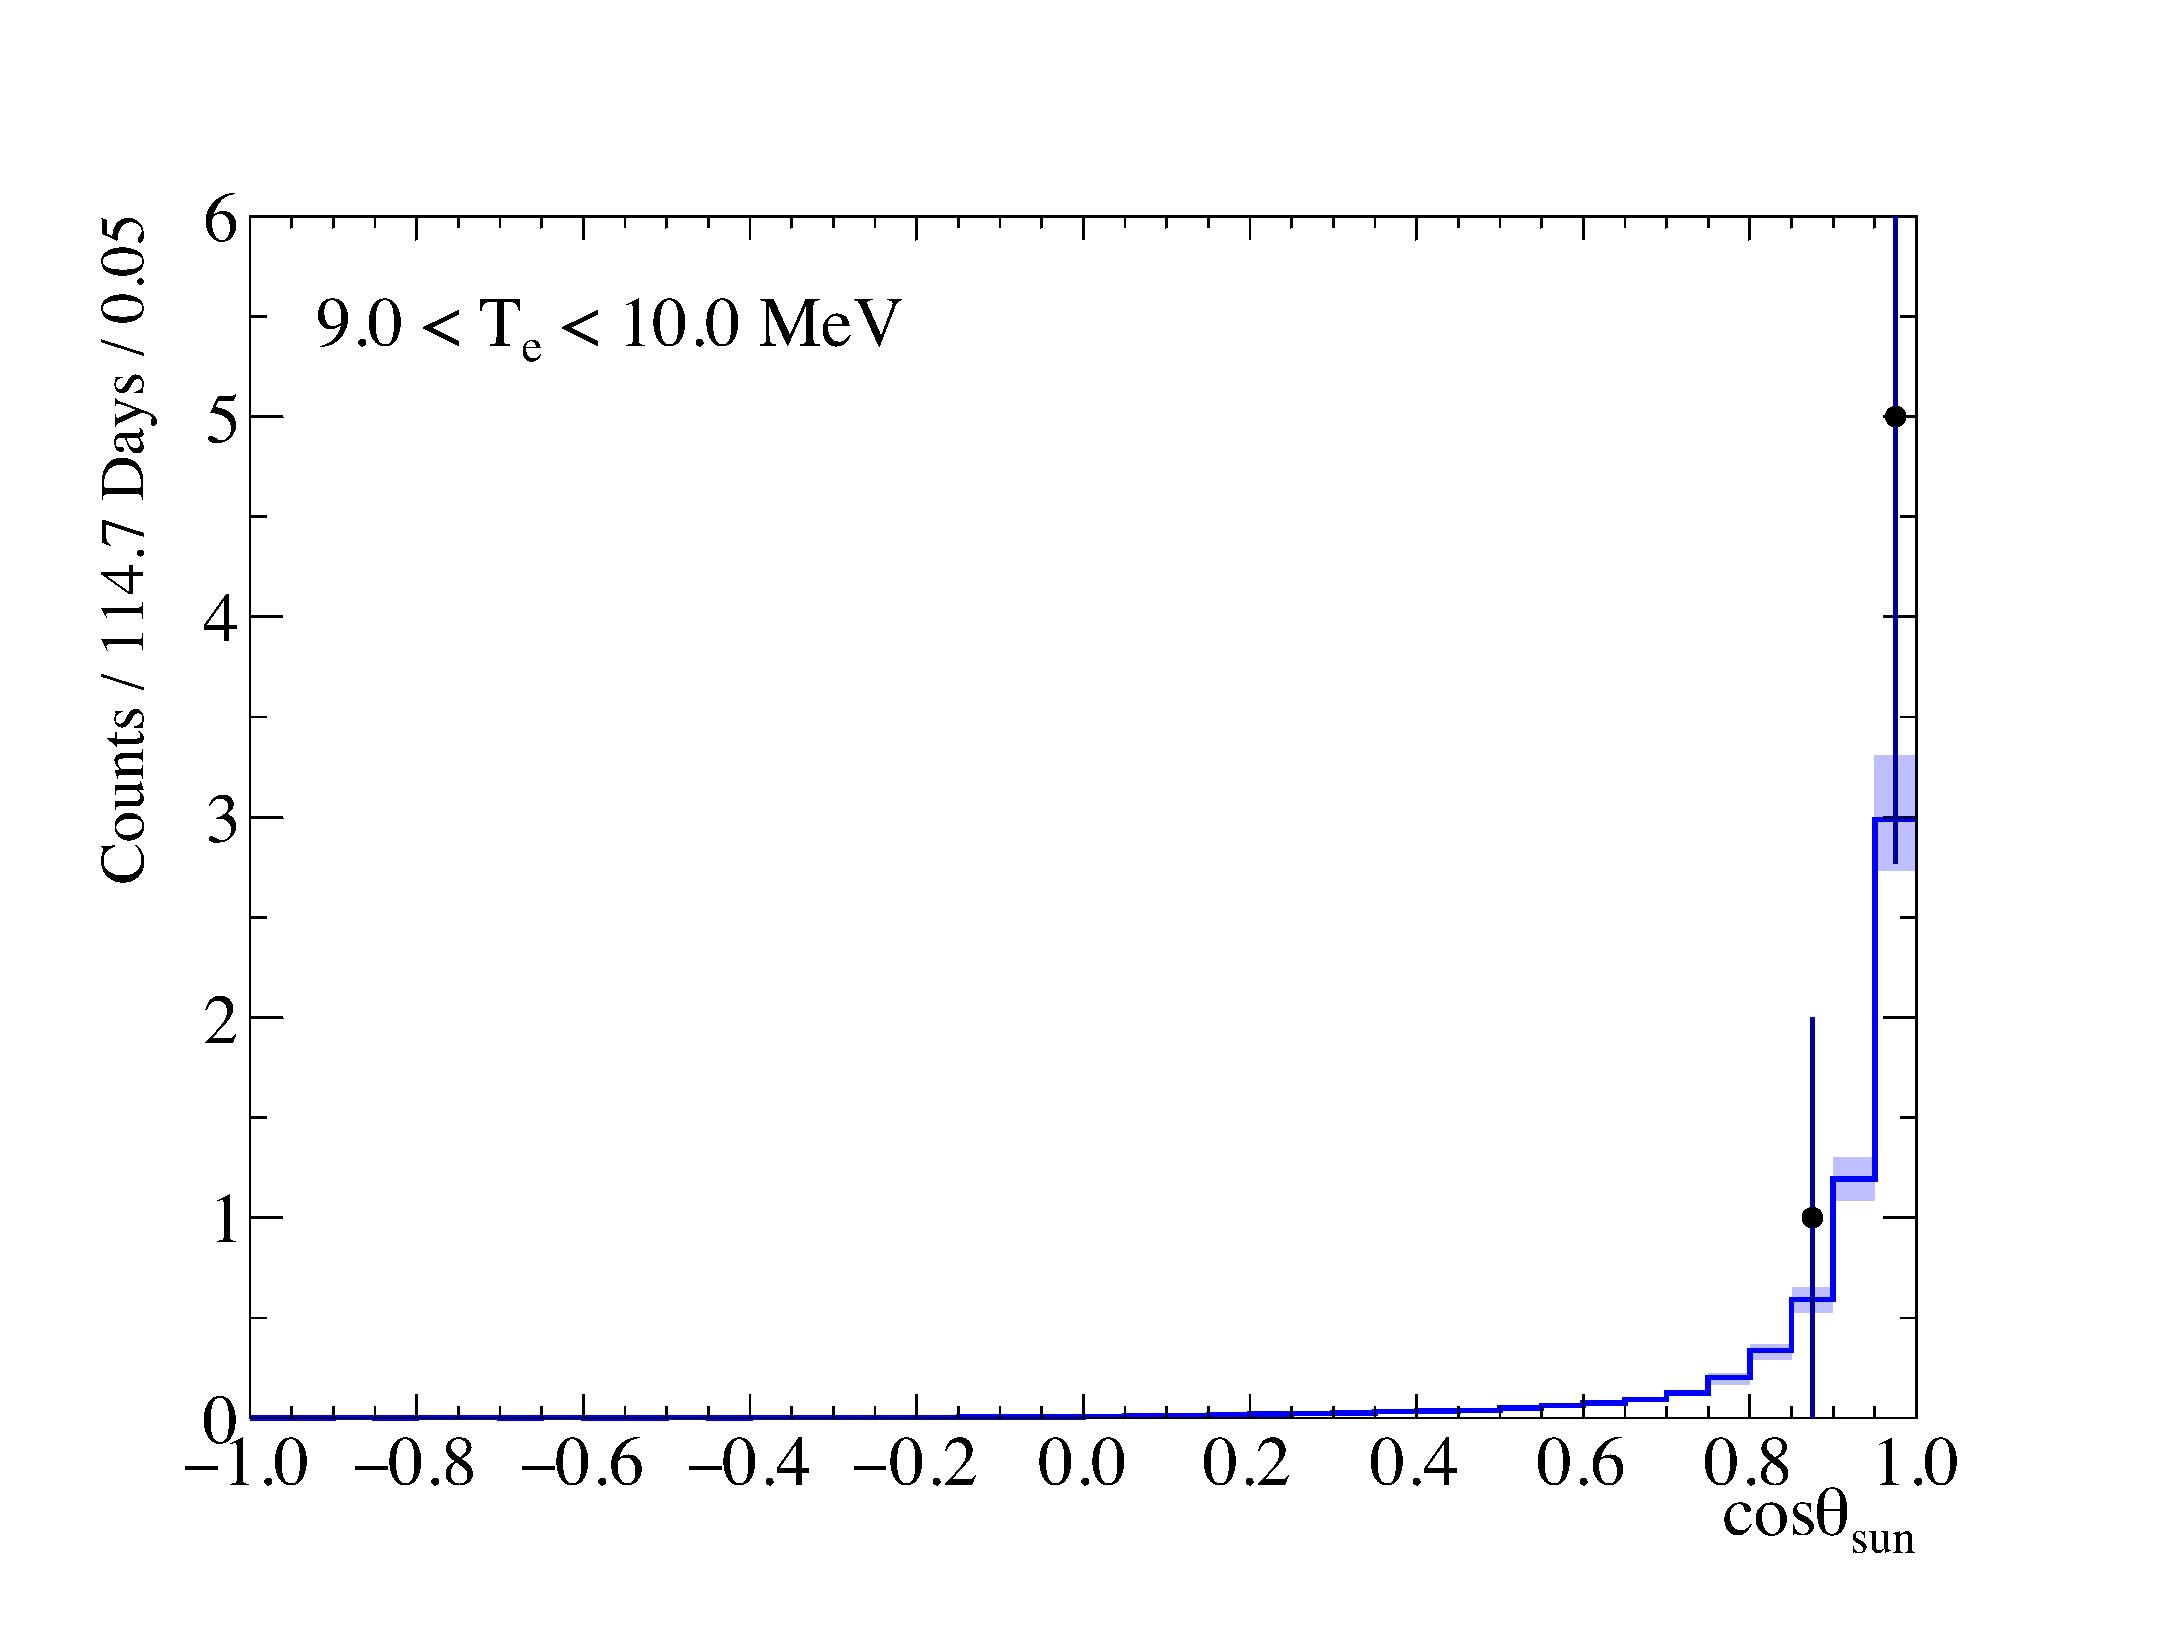
\includegraphics[width=\textwidth]{bin5}
\caption{}
\end{subfigure}
\hfill
\begin{subfigure}[b]{0.48\textwidth}
\centering
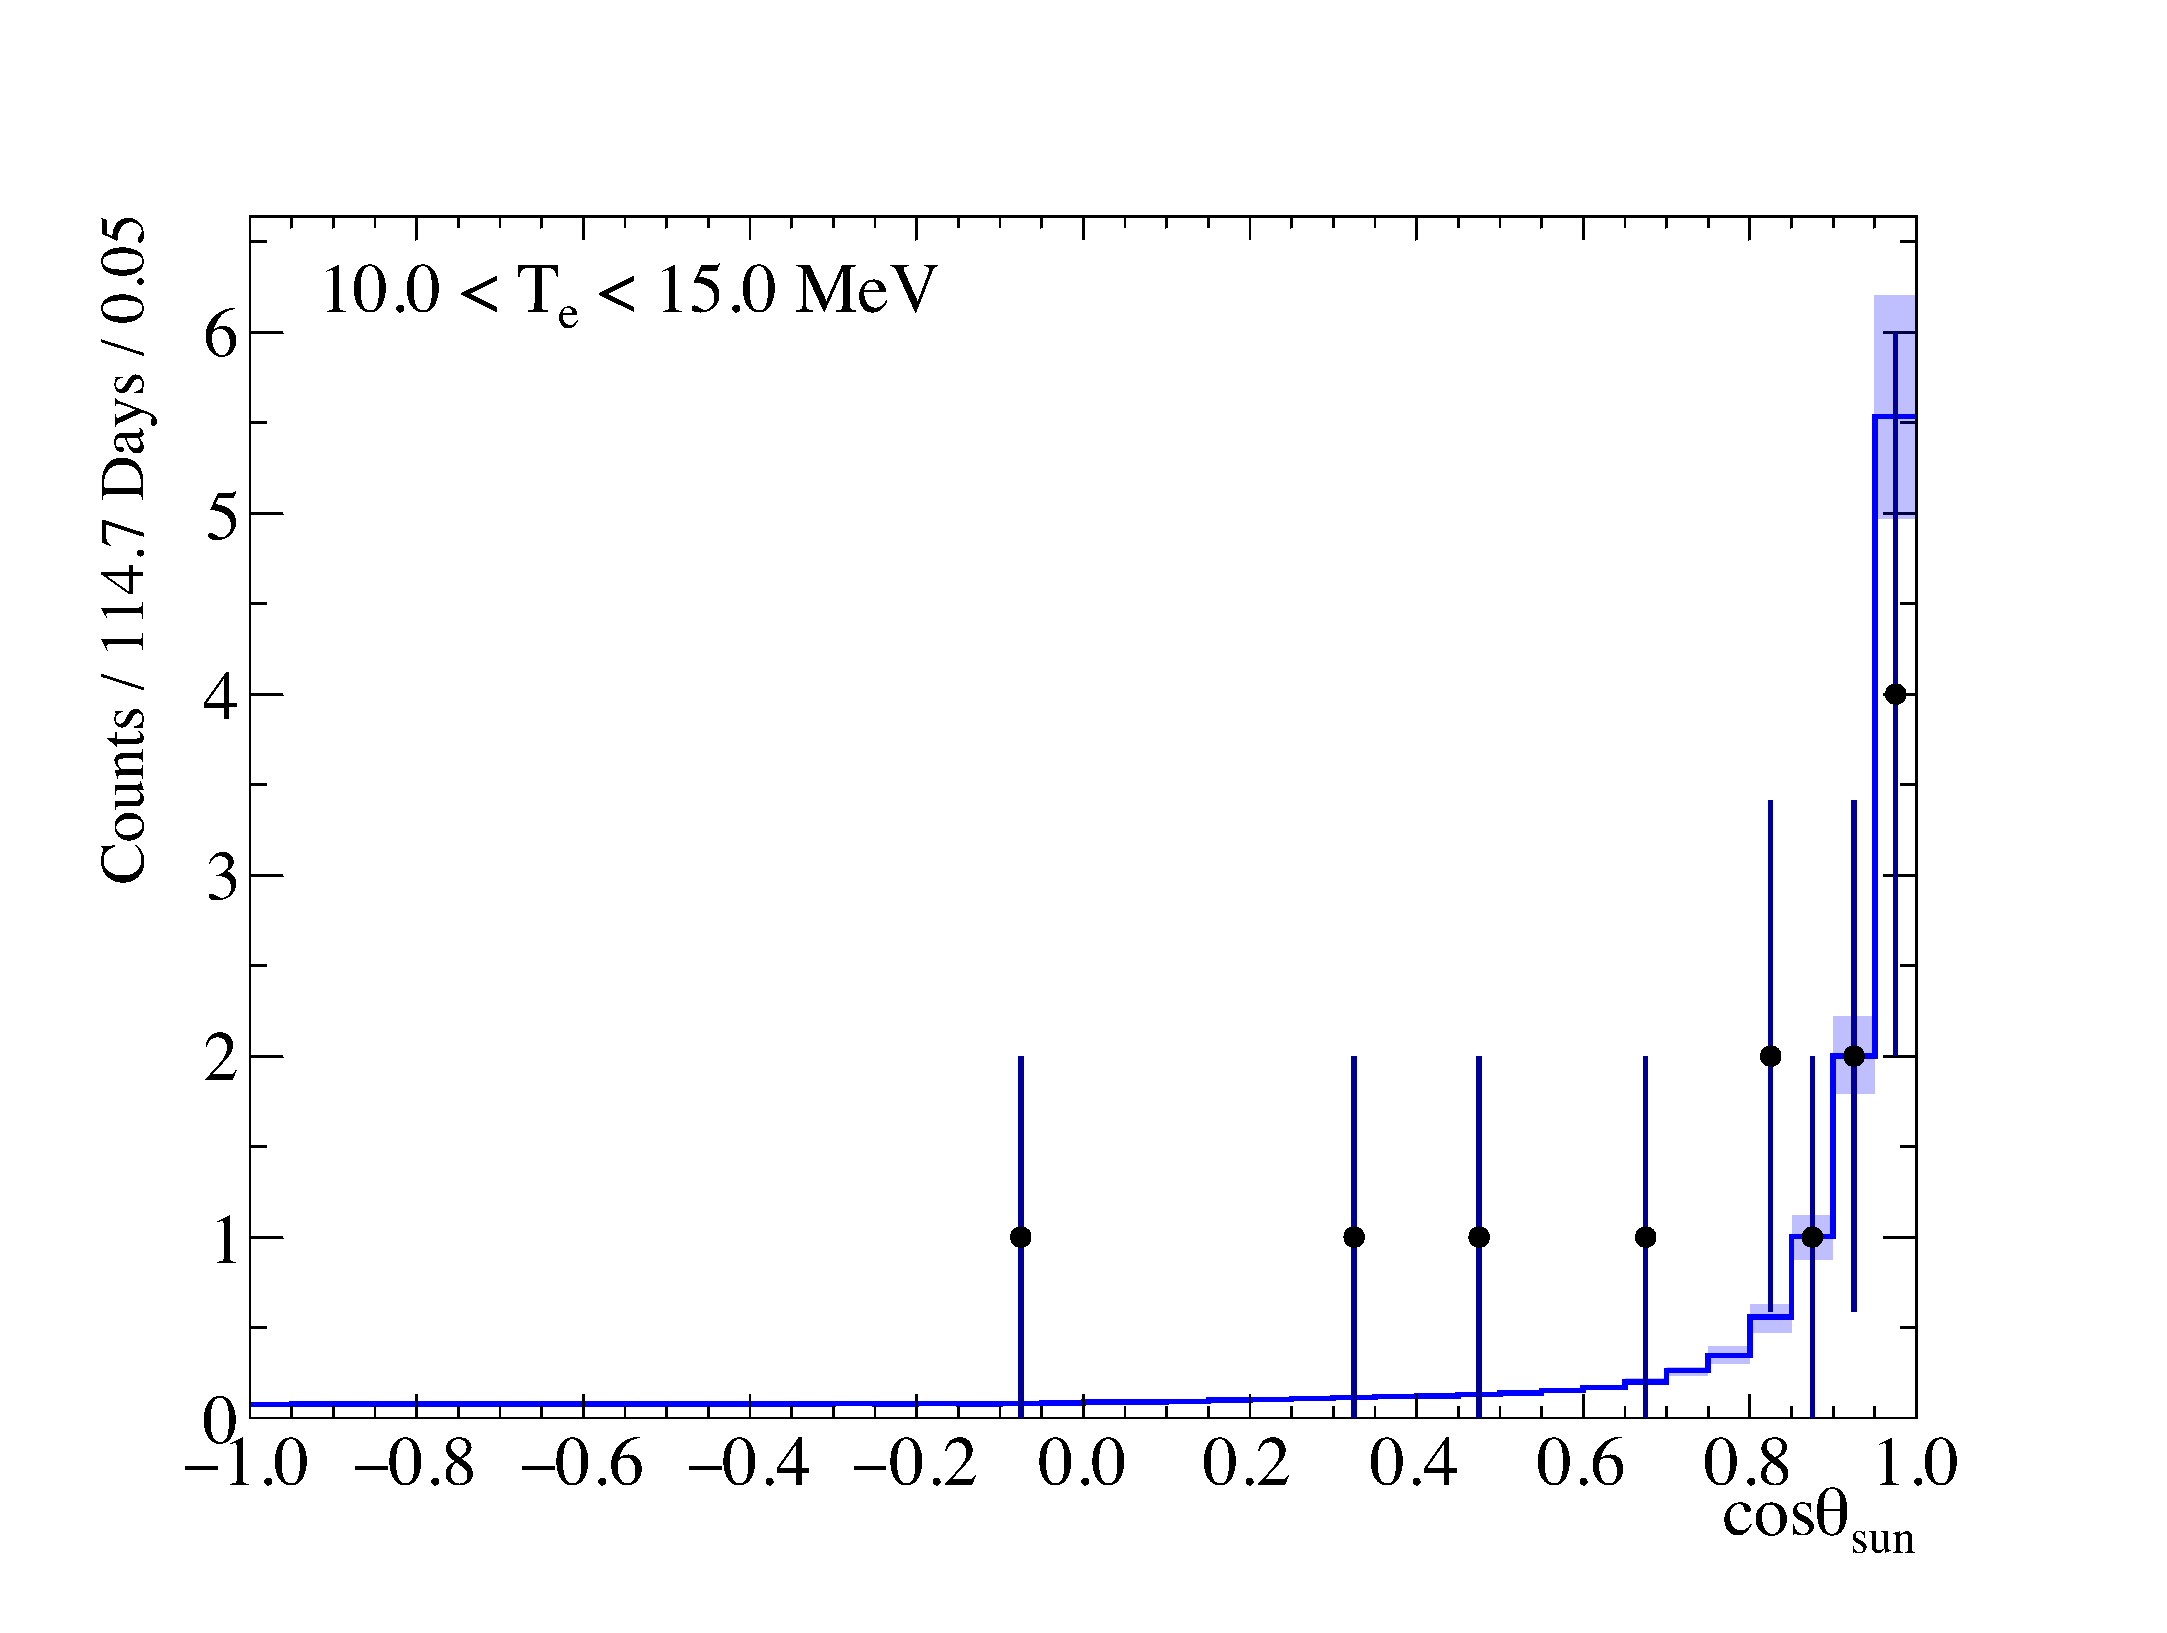
\includegraphics[width=\textwidth]{bin6}
\caption{}
\end{subfigure}
\caption[Bin-by-Bin $\cos\theta_{sun}$ Distributions]{
Distribution of events in $\cos\theta_{sun}$ in all six energy bins with
best fit signal+background distribution.}
\label{fig:binbybin}
\end{figure}

\section{Outlook For Water and Scintillator Phase}
The primary result of this analysis is a measurement of the $\ce{^{8}B}$
flux with the SNO+ detector. 
But, by using the $\ce{^{8}B}$ flux measured by the SNO experiment, the data for
this analysis can be used to measure the solar survival probability instead
of the flux.
This analysis is statistically limited, so a measurement of the survival
probability done this way would have uncertainties much larger than the similar
measurements done by the Super Kamiokande collaboration.
But, the low backgrounds observed at higher energies could allow for a good measurement
of the day-night effect once more data are acquired.
A measurement of the day-night effect could allow for relatively
competitive constraints on the standard neutrino mixing parameters.

Since the completion of this measurement SNO+ has acquired approximately double
the livetime, with lower backgrounds.
The decreased background rates may allow for an expanded fiducial volume at
higher energies, which would increase the available statistics for this measurement
or a possible measurement of the day-night effect.
A likelihood fit in both $\cos\theta_{sun}$ and radius might allow for an
expanded fiducial volume as well.

\begin{figure}[htbp]
    \centering
    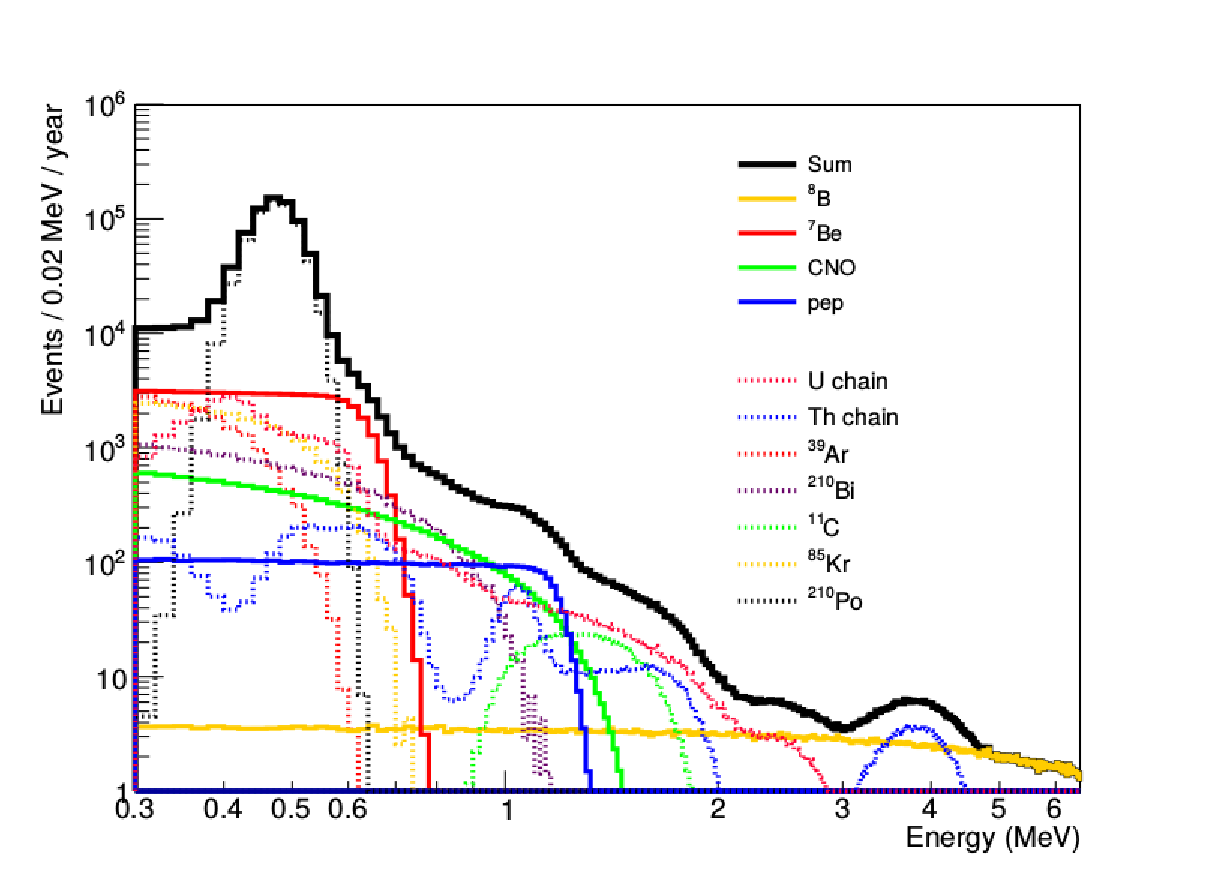
\includegraphics[width=0.78\textwidth]{globalfit_spectrum}
    \caption[Expected Scintillator Phase SNO+ Solar Neutrino Spectrum]{Expected interaction
    rates for solar neutrinos and backgrounds in SNO+'s scintillator phase}
    \label{fig:snop_scintillator}
\end{figure}
SNO+ has begun it's partial fill
period, in which the AV  water is replaced with liquid scintillator.
Once complete SNO+ will be able to take data for low-energy solar neutrino
analysis.
The expected increase in radio-purity and energy resolution will allow
for solar neutrinos to be identified above background at much lower energies
than was possible in the water phase.
Figure~\ref{fig:snop_scintillator} shows the expected solar neutrino and
background spectrum at low energies for SNO+, scintillator purity related
backgrounds are assumed to be at Borexino levels.

One of SNO+'s advantages for making solar neutrino measurements is the
very large overburden, which provides a low rate of cosmogenic 
muons passing through the detector, which results in a low rate of
cosmogenic isotope production within the detector.
One of the most significant cosmogenic isotopes for low energy solar is
the $\ce{^{11}C}$, which has a half-life of 20\,minutes and produces a
$\beta^{+}$ with an endpoint energy approximately $1$\,MeV.
The long half-life means the $\beta^{+}$ cannot easily be associated with
the muon that produced it, and the energy spectrum for the decay is at
the end point for the $pep$ and CNO solar neutrino fluxes.
So a low rate of cosmogenic muons will mean the $\ce{^{11}C}$ background
does not preclude a significant measurement of the $pep$ and CNO neutrino flux.
However, the low rate of CNO neutrinos compared to $pep$ neutrinos and other
backgrounds will
still make a strong measurement of the CNO flux  very difficult.
With 6\,months of scintillator data it's expected that SNO+ will be able
to measure the $pep$ flux to $13\%$ uncertainty, almost a factor of two
improvement on existing measurements.
With the same data a measurement of $\ce{^{7}Be}$ flux to $5\%$ and the
$\ce{^{8}B}$ flux to $10\%$ is expected.

%\subsection{Mixing Results}
%By using the SNO $\ce{^{8}B}$ flux result as the true value for the full,
%flavor independent, $\ce{^{8}B}$ solar neutrino flux, this measurement of the
%solar elastic-scattering rate can be used to the effective solar neutrino survival
%probability.
%This sort of measurement has been done before, most significantly by
%Super Kamiokande~\citep{superk1,superk2,superk3,superk4}.
%%and also by Borexino???TODO check if borexino has doen this
%
%For any combination of electron recoil energy $T_{\mathrm{e}}$ and solar
%neutrino energy, $E_{\nu}$ the relation between the survival probability
%and the elastic scattering rate is........
